\documentclass[onecolumn]{sig-alternate-10pt-onecolumn}
%\documentclass[conference,onecolumn,10pt]{IEEEtran} 

\usepackage{color}
\usepackage{multirow}
\usepackage{url}

\usepackage{algorithm}
\usepackage[noend]{algpseudocode}
\usepackage{enumitem} % for concise list env
\usepackage{subfigure}
\newcommand{\myitem}[1]{\vspace*{0.03in}\noindent\textbf{#1}}
\newcommand{\afteritem}{\vspace*{0.07in}}

\newcommand{\xin}[1]{\textcolor{red}{(XIN: #1)}}
\newcommand{\jrex}[1]{\textcolor{blue}{(JREX: #1)}}
\newcommand{\el}[1]{\textcolor{blue}{(EL: #1)}}
\definecolor{Ora}{cmyk}{0, 0.6, 0.8, 0}
\newcommand{\lv}[1]{\textcolor{Ora}{(LV: #1)}}
\newcommand{\cut}[1]{}

%\widowpenalty 10000
%\clubpenalty 10000

\vspace{-1.7in}
\title{MAZU: Taming the Long Tail Latency \\in Software Defined Networks}

%\numberofauthors{1}
\author{
%TODO: add the rest
Keqiang He$^\dagger$ \hspace{0.02in} 
Sourav Das $^\dagger$ \hspace{0.02in} 
Junaid Khalid$^\dagger$ \hspace{0.02in} 
Aditya Akella$^\dagger$ \hspace{0.02in} 
Li Erran Li$^\star$ \hspace{0.02in} 
Marina Thottan$^\star$ \hspace{0.02in} \\
%\affaddr{
Bell Labs, Alcatel-Lucent$^\star$ \hspace{0.1in}
University oF Wisconsin$^\dagger$ \hspace{0.1in}
}
%\alignauthor Internal Discussion
%\alignauthor Internal Discussion\\
%       \affaddr{Department of Computer Science}\\
%       \affaddr{Princeton University}\\
%       \email{xxx@cs.princeton.edu}
%}

\begin{document}
\maketitle

\vspace{-0.7in}
\section{Latency Between Control Plane and Data Plane}
\label{sec:intro}
%Software defined networking has been envisioned to be deployed in a variety of
%settings such as data centers, cellular networks, wide area networks.
%{Proposals for employing SDN in a variety of settings: WAN, DC, mobile. Openflow
%  is a common and popular API in these settings. expand} 
%\subsection{Need for low latency}
%\begin{figure}[b]
%\centering
%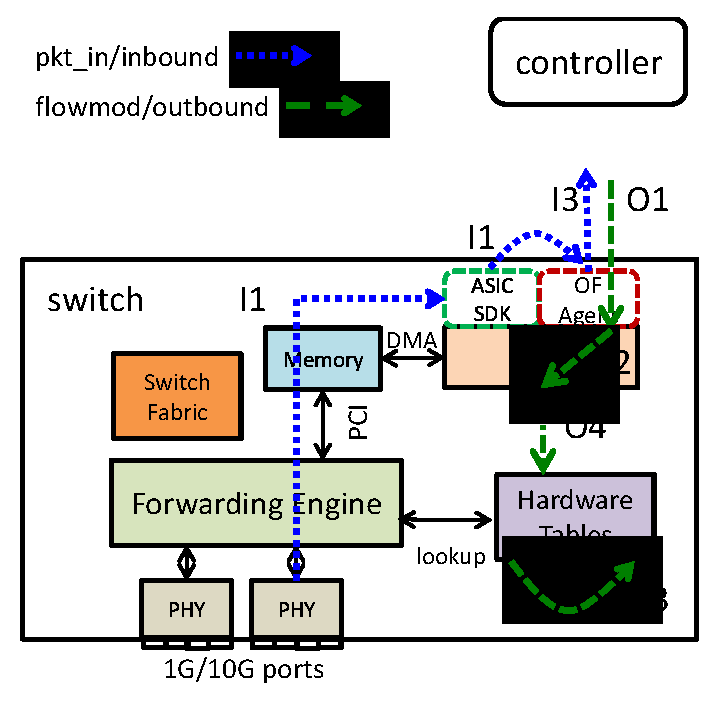
\epsfig{file=./figs/openflow_switch_illustrate.eps,width=0.3\textwidth}
%\caption{Illustration of the t\_in and t\_out delay in an openflow switch.}\label{openflow_switch_delay}
%\end{figure}

\begin{figure*}[b]
\centering
%\vspace*{-0.23in}
\subfigure[Switch Architecture]{
\label{fig:switch}
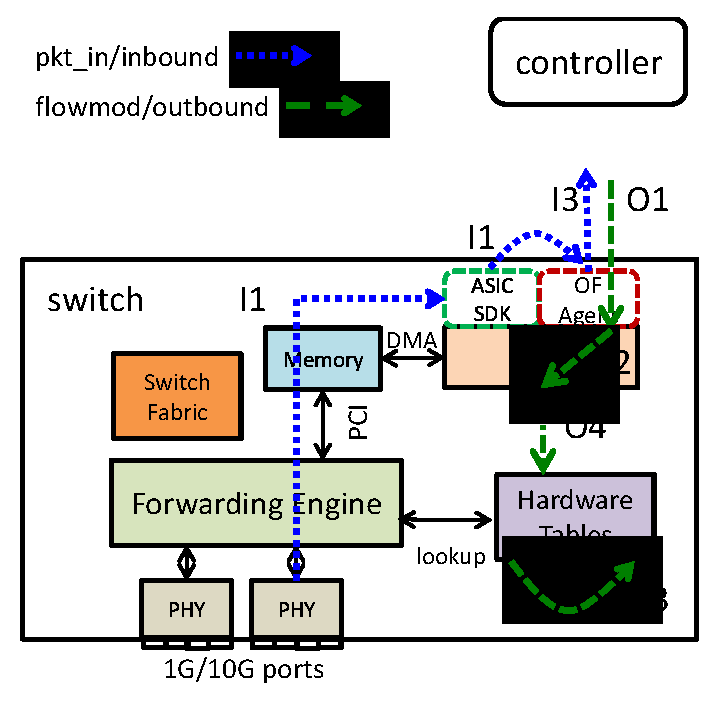
\includegraphics[width=1.5in]{./figs/openflow_switch_illustrate.eps}}
\hspace{-0.15in}
\subfigure[Mazu Framework]{
\label{fig:framework}
\includegraphics[width=2.in]{./figures/Mazu-arch.png}}
\hspace{-0.25in}
\subfigure[Insert bursts of low priority rules into a table with 100 high priority rules]{
\label{fig:result1}
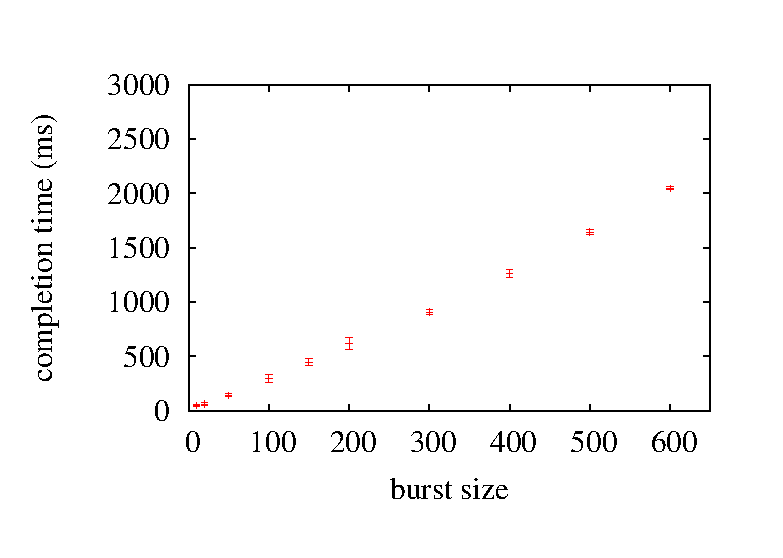
\includegraphics[width=1.7in]{./figs/bcm_two_pri_high_100_low_burstB.eps}}
%\hspace{-0.1in}
\subfigure[Insert bursts of high priority rules into a table with 100 low priority rules]{
\label{fig:result2}
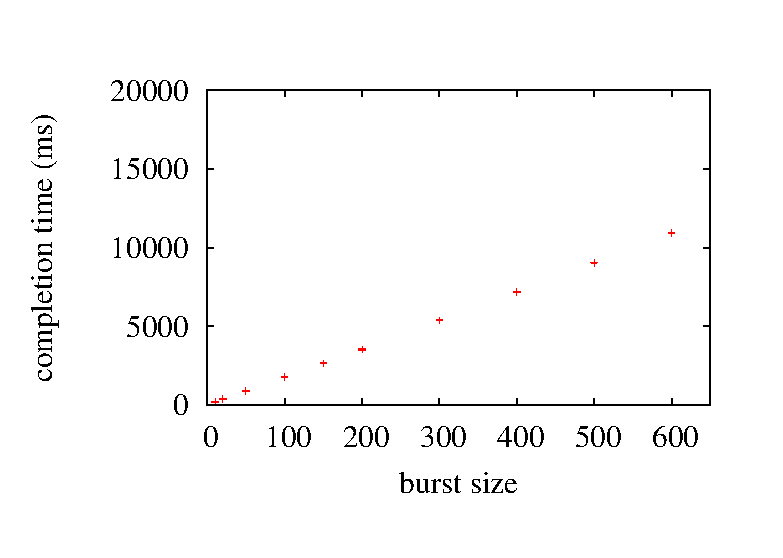
\includegraphics[width=1.7in]{./figs/bcm_two_pri_low_100_low_burstB.eps}}
\vspace*{-0.15in}
\caption{Switch, Mazu Architecture, and Measurement Results}
\vspace*{-0.1in}
\label{fig:mazu}
\end{figure*}
How quickly can a logically centralized controller manage and control the data
plane is crucial to many important network functions such as failure recovery,
reliability, fine-grained traffic engineering, and mobility in cellular
networks. For example, when failure occurs, to minimize network disruption, the
controller needs to quickly reroute impacted traffic. Network reliability is
greatly improved if data plane events are processed quickly. To handle fast
changing traffic patterns in data center networks, there is a need to perform
fine-grained traffic engineering every few seconds. To enable seamless mobility,
paths have to be setup fast.   
 
\subsection{Dissecting the latency}
However, recent measurements~\cite{ucsdHiFi13} have shown that the latency between control plane
and data plane is actually very large. OpenFlow rules can only be installed in a
slow rate of several hundreds per second. 
In Figure~\ref{fig:switch}, we show a simplified view of an SDN switch,
various actions the switch takes and how they contribute to the inbound delay,
which is defined to be the latency from the time a packet leaves switch
data plane to the time it arrives at the controller, and the outbound delay,
 which is defined to be the latency 
from the time the flow\_mod message leaves the controller to the time that
the corresponding rule gets installed in switch hardware. As
the figure indicates, the inbound delay and outbound delay depend on key aspects of
the switch's design including how the switch software processes different
messages, the software's interaction with the switch hardware table (typically a
TCAM), and the corresponding actions taken by the hardware table's SDK.  These
aspects may be exercised to different extents based on switch workload, such as
the nature of the rule being installed (simple 5-tuple based vs complex rule
based on the entire OpenFlow 10-tuple), the rule's priority relative to those
already installed, size of the currently installed rule base, rate at which the
controller is simultaneously pushing other rules to the switch and the nature of
those rules, etc. 

For example, as shown in Figure~\ref{fig:result1} and~\ref{fig:result2} if we
install bursts of low priority rules into a table with 100 high priority rules,
the completion time for 600 rules is around 2 sec. However, if we install bursts
of high priority rules into a table with 100 low priority rules, the completion
time for 600 rules is more than 10 sec. This is because the second case triggers
TCAM reordering.

To date, not much attention has been paid to estimating these latencies in the
wild under various workloads, and understanding the impact of switch
designs.  Understanding these is crucial to how SDN is used: it can inform
operators on whether certain SDN approaches (such as reactive failure recovery,
i.e. no fast reroute in data plane) can offer close to the promised benefits
given current switches on the market.  It can also inform then on how to avoid
or mitigate the impact of the latencies. To switch and chip vendors, it can
highlight what aspects of their software and SDK designs can be improved to
support faster actions. 
% how to alter SDN switch designs where possible to address the latencies, and how to develop SDN applications that modulate switch workloads to avoid being impacted by the latencies.



\section{Mazu Design}
We present, Mazu, a systematic framework that addresses latency problems
comprehensively. 
%how a network that has
%deployed SDN can overcome the impact of the latencies described in the
%previous section on various key management applications. 
Our goal is to develop a general set of approaches that work across most if not
all applications and deployment settings. 
%Our ultimate goal is to
%ensure applications meet the goals they were designed for as
%effectively as possible.
As shown in Figure~\ref{fig:framework}, Mazu controller implements a number of
modules. The Middlebox module handles inbound delay. The multipath probing
module sets up multiple paths in parallel. Data plane packets can flow through as
soon as the first path completes installation. This handles variable delay in
switch updates. The rule offloading module offloads rules to neighboring
switches to reduce latency. The optimal rule update module tries to update
switches as fast as it can.

\subsection{Inbound delay}
%We present a novel middlebox that isolates the processing of packet\_in messages
%from other actions on the switch, thereby almost eliminating t\_in. A network
%operator can deploy such middleboxes adjacent to ingress switches in her
%network.
For packet\_in processing, 
To elaborate, a packet typically follows these steps at the switch: 1)
arrives at port and is processed by ASIC, 2) ASIC decides to send "to
CPU" across PCI bus, 3) OS interrupt is raised and ASIC SDK gets
packet, 4) switch-side openflow agent wakes up, processes packet, and
puts on socket to controller.

%a packet typically follows the following steps at the
%switch: 1) arrives at the switch port and PHY, 2) is processed by ASIC, 3) ASIC decides to send "to CPU", 4)
%packet goes across PCI bus to CPU, 5) OS interrupt is raised and handled, 6)
%ASIC SDK gets packet and fires it off to a dispatch hook, 7) switch-side
%openflow agent wakes up, pro- cesses packet, and puts on socket to
%controller. 

Steps 1 to 4 are typically quite fast. The latencies we observe are mainly due to
steps 5 to 7. Earlier measurements show that steps 5 to 7 are slow due to
unoptimized switch implementations. Our measurements indicate that the newer
switches we measured have better implementations of these steps, but latency
arises nevertheless due to contention between simultaneous processing of
packet\_in messages along- side packet\_out flow\_mod and flow statistics
polling messages being received from the controller. 
 
To overcome the inbound latency entirely the key insight we leverage is to
physically decouple the switch's handling of packet\_in and packet\_out messages
from flow\_mod messages. We punt all packet\_in message generation and packet\_out
processing to a separate optimized processing unit, e.g., simple middlebox,
adjacent to the switch. We establish a (short) label-switched path between the
switch and its corresponding middlebox. The switch continues to have a control
channel to the controller (an SSL connection); in addition, we establish a
control channel (SSL) between the middlebox and the controller. The controller
must be aware of the middlebox's presence and must associate it with the
relevant switch. 

To exercise the middlebox, we insert a default low priority rule in the
switch; this helps redirect all unmatched packets on the label-switched path
to the middlebox. The middlebox generates the necessary
packet\_in messages and forwards them on its control channel to the
controller. The controller sends packet\_out messages to the middlebox; the
middlebox process the message and forwards the corresponding data packet to the
switch for further forwarding to the eventual destination. 
%flow\_mod messages directly to the switch. 

\subsection{Outboud delay}
%Ideally, the approaches we propose must avoid the latencies altogether
%to ensure that the applications can be supported effectively. We show
%that this is possible to achieve for inbound delay. However, 
Because
the underlying causes of outbound delays are tightly linked with how
the switches processes and stores forwarding rules, we can hope at
best to mitigate these latencies, and complete avoidance is
impossible. We develop a multi-step approach to maximally mitigate the impact on
outbound delay of various factors we have discovered.

First, we propose flow engineering that attempts to control the aggregate number
of rules inserted at any switch while adhering to the objectives of the
application(s) running. As such, this technique has to be implemented within the
application itself, although, we present a general framework for introducing
flow engineering into a given SDN applications. Flow engineering helps
upper-bound the aggregate impact of steps 1 and 2 above on any given switch. 

Second, we propose rule offload, where a subset of the rules to be installed at
a switch are carefully offloaded to downstream switches/routers having
sufficient capacity to hold the rules. This provides two advantages: (a) it
further reduces the number of rules installed at any switch. (b) The updates can
be executed in parallel thereby improving the overall time for insertion. 

Third, we propose priority ordered insertion, where the rules computed for
insertion at a switch are reordered into a sequence that is optimal with respect
to the switch's memory management scheme. This techniques mitigates the impact
of step 3. 

Fourth, for a given flow, we can setup multiple paths in parallel. Data plane
packets can go through as soon as the first path completes setup.

\iffalse
We develop a multi-step
approach to maximally mitigate the impact on t\_out of various factors we have
discovered. First, we present a novel "flow engineering" technique that optimizes
the number of new rules to be inserted at any switch while adhering to overall
network management objectives and flow table size contraints. We enhance this
using an "opportunistic rule offload" scheme that carves out subsets of rules to
be installed at edge-switches, taking into account rule dependencies, and
schedules them for installation at nearby core switches that have low flow
table occupancy. Finally, we control the actual installation of flows at edge
and core switches by reordering them according to priority.
\fi

\small
\bibliographystyle{ieeetr}
\bibliography{refs.bib}

\end{document}


% LocalWords:  Mazu OpenFlow SDN TCAM SDK tuple analying Middlebox multipath
% LocalWords:  optimial PHY ASIC PCI openflow cesses middlebox SSL middlebox's
% LocalWords:  Outboud multi contraints greybox XXXXms Broadcom chipset XXXs
% LocalWords:  rearrangment differentiator middleboxes multipronged
